\section{Dynamische Systeme}

\textbf{Fixpunkt:} $x^*:$ \hspace{1cm}$f(x^*) = 0$

\subsection{Gleichgewichtslösungen}
Die Gleichgewichtslösungen sind diejenigen Punkte, in welchen die Ableitung verschwindet:
\begin{equation*}
	\diffp{}{t}y(t) = 0
\end{equation*}
\subsection{Phasengerade und Integralkurven}
Bei der Phasengerade werden die Gleichgewichtslösungen in Funktion der Ableitung eingetragen. Dadurch kann die Stabilität eines Systems bestimmt werden. 

\subsection{Eindimensionale Syteme}
Falls $x^*$ ein \textbf{Fixpunkt} von $\dot{x} = f(x)$ ist, ist $x(t) = x^*$ eine konstante Lösung des Systems $\dot{x} = f(x)$. Der \textbf{Phasenraum} eines eindimensionalen Systems vom Typ $\dot{x} = f(x)$ is $\mathbb{R}$. Wegen des \textbf{Eindeutigkeitssatzes} hat $\dot{x} = f(x)$ für alle $0 \leq t$ das selbe Vorzeichen. Die Lösung ist daher monoton steigend, monoton fallend oder ist ein Fixpunkt. Nur für \textbf{autonome} DLG 1. Ordnung sind keine periodische Lösungen möglich.

\subsection{Lineare Stabilitätsanalyse}
\label{sec:linStab}
$\eta (t) = x(t) - x^*$ \hspace{1cm} falls $x^* \neq 0 \Rightarrow$ Taylor:\newline
$\dot{\eta} = \dot{x} = f(x) \approx f(x^*) + f'(x^*) \cdot \underbrace{(x - x^*)}_{\eta (t)}(x - x^*) = f'(x^*) \cdot \eta$ \\
$\Rightarrow \mathrm{DGL}: \dot{\eta} = \eta \cdot f'(x^*),$ \hspace{1cm} $\eta(t) = \eta(0) \cdot e^{f'(x^*)t}$ \\ \\

\begin{tabular}{ll}
	\textbf{stabil:} \quad & $f'(x^*) < 0$ \\
	\textbf{instabil:} & $f'(x^*) > 0$ \\
	\textbf{(in)stabil:} & $f'(x^*) = 0$ \\
\end{tabular}\\ \\

\begin{multicols}{2}
	\subsection{Bifurkationen}
	
	\begin{equation*}
		\dot{x} = f(x,r), \quad r \in \mathbb{R}
	\end{equation*}
	
	Eine qualitative Änderung der Dynamik eines von einem Parameter $r$ abhängigen Systems, heisst Bifurkation. Die Parameterwerte von $r$ an denen diese qualitativen Änderungen erfolgen, heissen \textbf{Bifurkationspunkte} des Systems.
	\columnbreak
	\subsubsection{Saddle-Node-Bifurkation}
	Fixpunkte können durch Variation von $r$ erzeugt oder zerstört werden.
	
	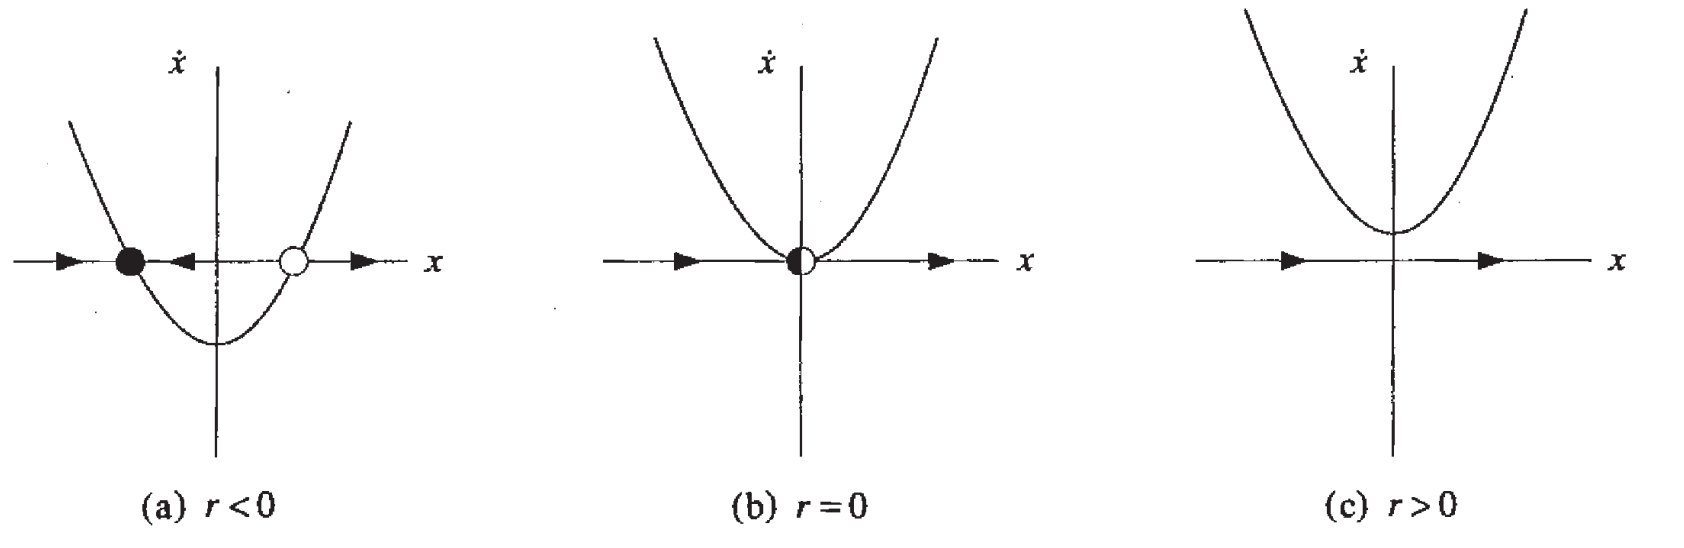
\includegraphics[width=0.5\textwidth]{./images/Saddle_Node.png}
\end{multicols}

\begin{multicols}{2}
	\subsubsection{Pitchfork-Bifurkation}
	Die Pitchfork Bifurkation ist eine Bifurkation, bei der ein Fixpunkt seine Stabilität änder und gleichzeitig zwei neue Fixpunkte entstehen. \newline \newline
	
	\textbf{superkritische Pitchfork-Bifurkation:} Man nennt diesen Typ von Bifurkation superkritisch, weil die Fixpunkte $x^* \neq 0$ nur für Parameterwerte \textbf{über} dem Bifurkationspunkt existieren, bzw. für $r >0$.
	
	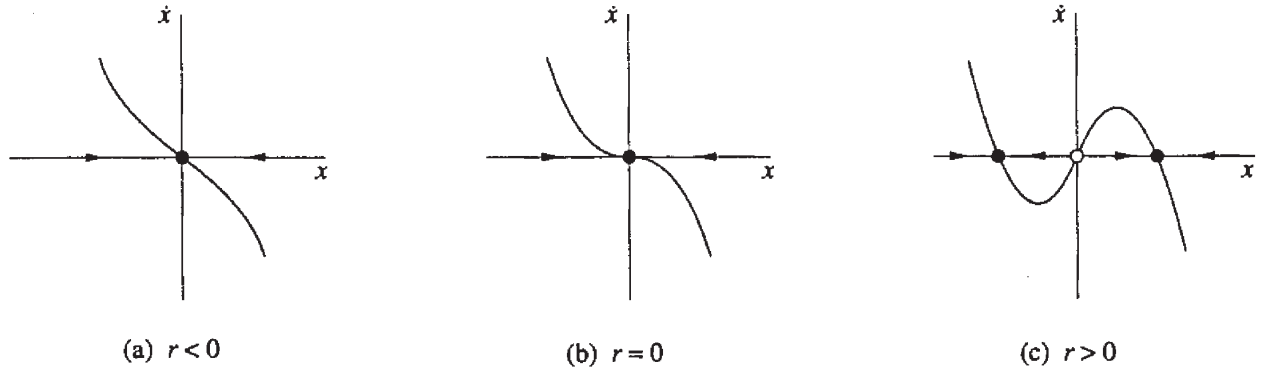
\includegraphics[width=0.5\textwidth]{./images/superkritisch.png}
	\columnbreak
	
	\textbf{subkritische Pitchfork-Bifurkation:} Man nennt diesen Typ von Bifurkation subkritisch, weil die Fixpunkte $x^* \neq 0$ nur für Parameterwerte \textbf{unter} dem Bifurkationspunkt existieren.
	
	\subsubsection{Transkritische Bifurkation}
	Bei einer transkritischen Bifurkation werden keine Fixpunkte erzeugt oder vernichtet, allerdings wird die Stabilität zweier Fixpunkte vertauscht.
\end{multicols}

\subsection{Bifurkationsdiagramm}
	Diagramm der kritischen Punkte in Abhängigkeit eines Parameters (e.g. $a$).
	
	Beispiel:
	
	\[y'=y(a-y)\]
	
\begin{tabular}{p{0.3\textwidth}p{0.3\textwidth}p{0.3\textwidth}}
	\vspace{0pt}	
	\begin{tabular}[h]{p{0.1\textwidth}p{0.2\textwidth}}
	Ausgezogen:		& Asymptotisch Stabil\\
	Gestrichelt:	& Instabil\\
	Zentrum:		& Semistabil\\
	\end{tabular}
	& 	\vspace{0pt}
		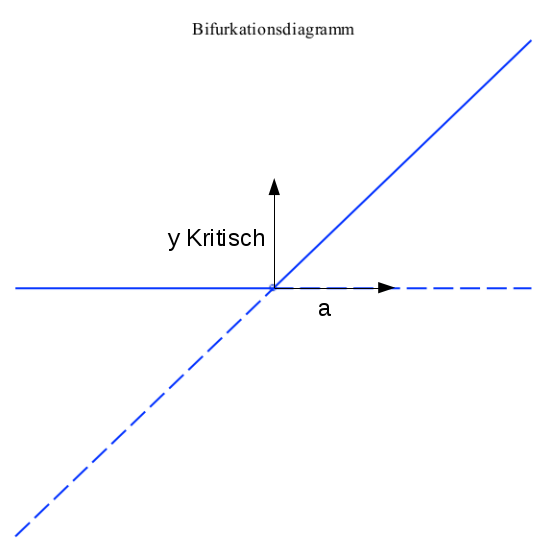
\includegraphics[width=0.3\textwidth]{images/Bifurkationsdiagramm.png}
	& 	\vspace{0pt}
		\textbf{Vorgehen:}
		\begin{tabular}[h]{p{0.02\textwidth}p{0.28\textwidth}}
		1:	& Kritische Punkte berechnen ($\dot{x} = 0$). Ergibt $x^*_k(a)$.\\
		2:	& Stabilität der Punkte berechnen (gemäss Section \ref{sec:linStab}).\\
		3:	& Kurven in Diagramm ($x^*(a)$ aufzeichnen).\\
		\end{tabular}\\
\end{tabular}

\subsubsection{Allgemein 1. Ordnung}
\[ \dfrac{d}{dt}y(t)=f(t,y(t)) \qquad y(t_0)=y_0 \]
Eindeutige Lösung $\varphi(t)$ im Intervall falls $f(t,y(t))$ und $\dfrac{d \; f(t,y(t))}{dt}$ stetig im Intervall.

\subsection{Zweidimensionale Systeme}

\begin{tabular}{ll}
	\textbf{stabil:} \qquad & $\lvert x(t) - x^*\rvert < \epsilon \quad 0 < t < \infty$ \\
	\textbf{instabil:} & $\lvert x(t) - x^*\rvert \nless \epsilon \quad 0 < t < \infty$ \\
	\textbf{asymptotisch stabil:} & $\lim\limits_{t \to \infty} \lvert x(t) - x^*\rvert = 0$ \\
\end{tabular}\\ \\

\subsubsection{Typen von Fixpunkten}

\begin{tabular}{ll}
	\textbf{Spur:} \qquad & $\tau = \mathrm{tr}(A) = a_{11} + a_{22} = \lambda_1 + \lambda_2$ \\
	\textbf{Determinante:} & $\Delta = \det(A) = a_{11}a_{22}  - a_{12}a_{21} = \lambda_1 \lambda_2$\\
	\textbf{Eigenwerte:} & $\lambda_{1,2} = \frac{1}{2} \left(\tau \pm \sqrt{\tau^2 - 4\Delta}\right)$ \\
\end{tabular}\\ \\

Für $\Delta > 0$ und $\tau < 0$ gilt: \\
\begin{tabular}{|p{5cm}|p{13cm}|}
\hline \textbf{Eigenwerte} & \textbf{Stabilität} \\ 
\hline $\operatorname{Re}(\lambda_1) < 0$ und $\operatorname{Re}(\lambda_2) < 0$ & stabiler Knotenpunkt ($\tau^2 - 4 \Delta > 0$ bzw. $ \lambda_1, \lambda_2 \in \mathbb{R}$) \\ 
 & stabiler Strudelpunkt ($\tau^2 - 4 \Delta < 0$ bzw. $ \lambda_1, \lambda_2 \notin \mathbb{R}$) \\
\hline 
\end{tabular} \\

Für $\Delta > 0$ und $\tau > 0$ gilt: \\
\begin{tabular}{|p{5cm}|p{13cm}|}
\hline \textbf{Eigenwerte} & \textbf{Stabilität} \\ 
\hline $\operatorname{Re}(\lambda_1) > 0$ und $\operatorname{Re}(\lambda_2) > 0$ & instabiler Knotenpunkt ($\tau^2 - 4 \Delta > 0$ bzw. $ \lambda_1, \lambda_2 \in \mathbb{R}$) \\ 
 & instabiler Strudelpunkt ($\tau^2 - 4 \Delta < 0$ bzw. $ \lambda_1, \lambda_2 \notin \mathbb{R}$) \\
\hline 
\end{tabular} \\

Für $\Delta > 0$ und $\tau = 0$ gilt: \\
\begin{tabular}{|p{5cm}|p{13cm}|}
\hline \textbf{Eigenwerte} & \textbf{Stabilität} \\ 
\hline $\operatorname{Re}(\lambda_1) = \operatorname{Re}(\lambda_2) = 0$ & Zentrum bzw. einen elliptischen Fixpunkt\\
\hline 
\end{tabular} \\

Für $\Delta = 0$ gilt: \\
\begin{tabular}{|p{5cm}|p{13cm}|}
\hline \textbf{Eigenwerte} & \textbf{Stabilität} \\ 
\hline $\lambda_1 = 0$ oder $\lambda_2 = 0$ & degeneriertes System; Fixpunkte sind nicht isoliert(bspw. ganze Gerade als Fixpunkte) \\ 
\hline 
\end{tabular} \\

Für $\Delta < 0$ gilt: \\
\begin{tabular}{|p{5cm}|p{13cm}|}
\hline \textbf{Eigenwerte} & \textbf{Stabilität} \\ 
\hline $\lambda_1 < 0 < \lambda_2$ & Sattelpunkt (saddle point) \\
\hline $\lambda_2 < 0 < \lambda_1$ & Sattelpunkt (saddle point) \\ 
\hline 
\end{tabular} \\

\textbf{Allgemein:}\\
\begin{tabular}{ll}
	\textbf{grenzstabil:} \qquad & $\operatorname{Re}(\lambda_i) \leq 0$ für alle $\lambda_i$ \\
	\textbf{instabil:} & $\operatorname{Re}(\lambda_i) > 0$ für mind. einen Wert \\
	\textbf{asymptotisch stabil:} &$\operatorname{Re} < 0$ für alle $\lambda_i$ \\
\end{tabular}\\ \\

\subsection{Atraktorbereich und Separatrizen}
Haben wir ein autonomes System mit Anfangswertproblem. Die Gesamtheit aller Punkte des Phasenraums - die als Anfangsbedingung gewählt - zu einer Trajektorie führen, welche dann gegen einen speziellen Punkt konvergiert, heisst Atraktorbereich des Punktes. 
Die Ränder, welche diese Bereiche trennen, heissen Separatrizen. 
Im Bild sehen wir zwei Atraktorbereiche, welche durch die beiden blauen Kurven (die Separatrizen) getrennt sind. 
Startet man innerhalb der Blase, so konvergiert man gegen den Punkt (0,0) ansonsten gegen den Punkt (1,-2). 
\begin{minipage}[h!]{0.35\textwidth}
	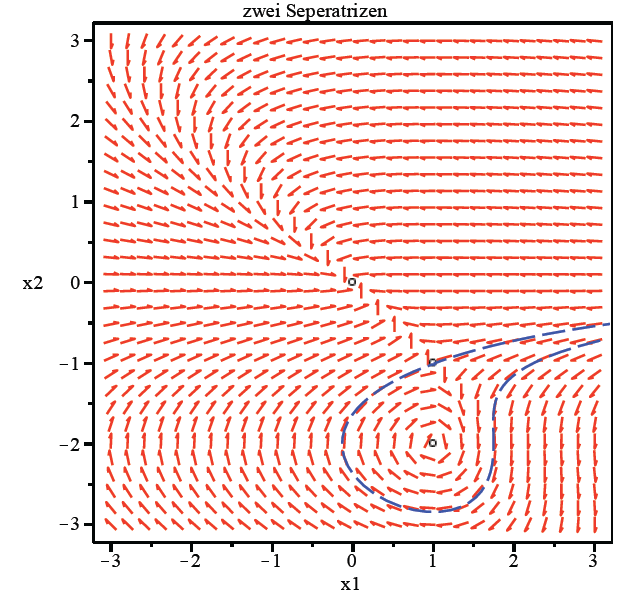
\includegraphics[width=1\textwidth]{images/Atraktorbereich.png}
\end{minipage}

\subsection{Vektorfeld und Trajektorie}
\begin{figure}[h!]
	\centering
	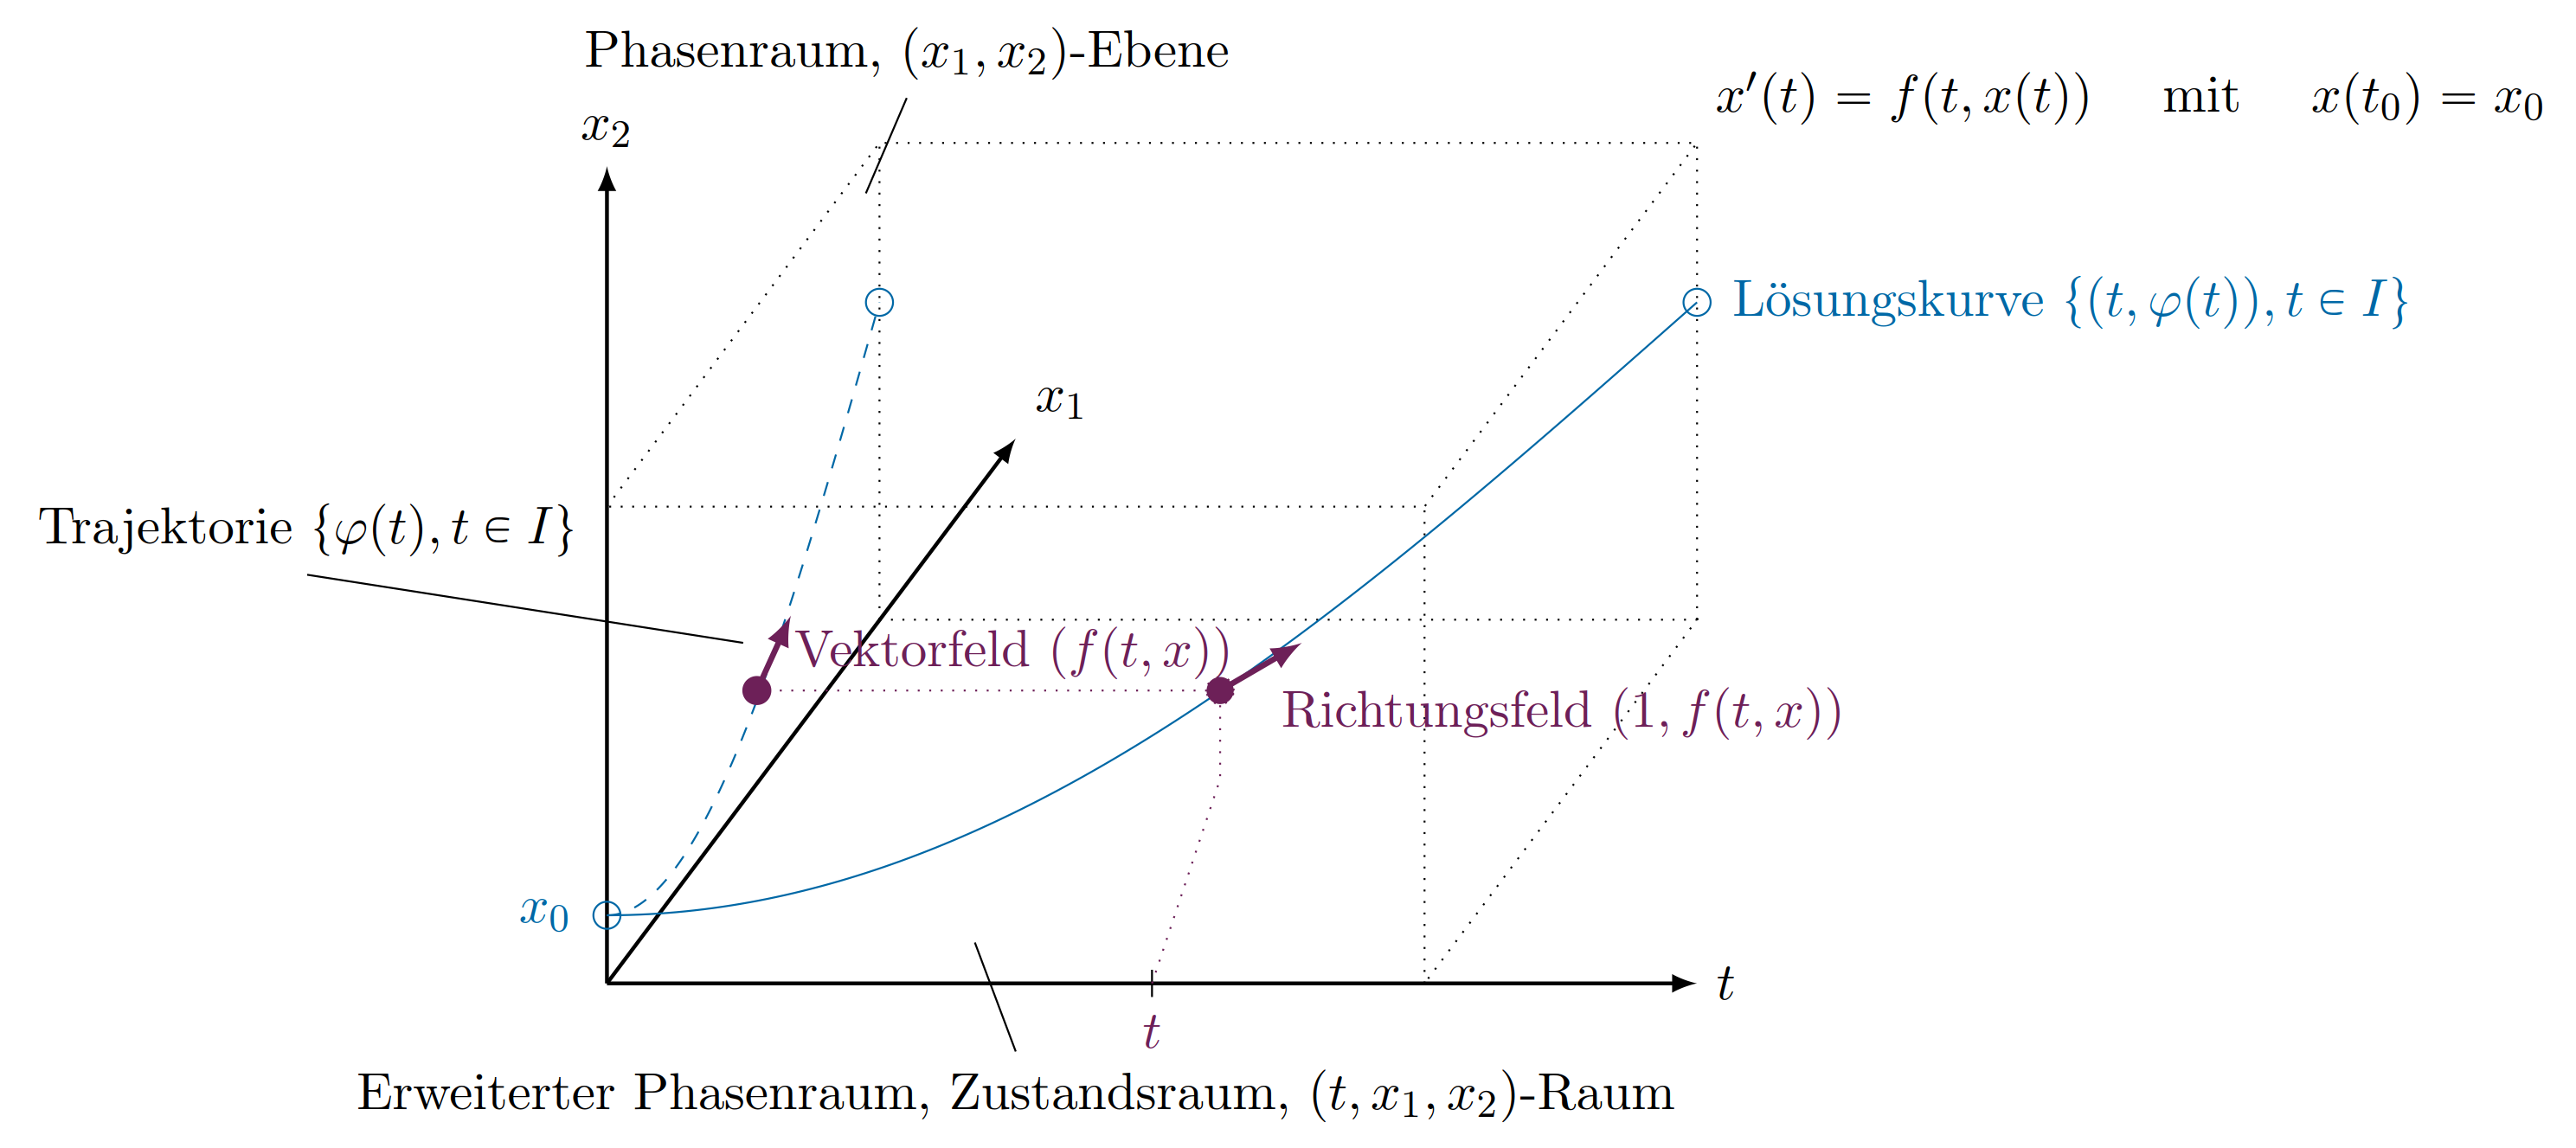
\includegraphics[width=0.8\textwidth]{./images/phasenraum.png}
\end{figure}


\subsection{Fast lineare Systeme, Jakobi-Matrix}
Ein System ist fast linear, wenn die Jacobimatrix $J_f$ regulär ist $det(J_f)\neq 0$. \\
\textbf{Robust:} Knotenpunkt, Studelpunkt, Sattelpunkt \\
\textbf{Marginal:} Zentrum, degenerierte Fälle \\ \\
1.Schritt: DGL in Form bringen:\\ 
$x'_1(t) = f_1(t) = x_2(t)$\\
$x'_2(t) = f_2(t) = -q(t)x_1(t)-p(t)x_2(t)+g(t)$\\
2.Schritt: Jacobi Matrix berechnen:\\
\begin{equation*}
	J_f(x) =    
	\begin{vmatrix} 
	        \frac{\partial f_1}{\partial x_1} & \frac{\partial f_1}{\partial x_2}\\ 
	        \frac{\partial f_2}{\partial x_1} & \frac{\partial f_2}{\partial x_2}\\   
	\end{vmatrix}
\end{equation*}
3. Schritt: Kritische Punkte berechnen (Ableitungen Null setzen...) $\rightarrow x^* = (x_{k1}^*, x_{k2}^*)$\\
4. Schritt: Jeden kritischen Punkt separat in die Jacobimatrix einsetzen\\
5. Schritt: Anschliessen für jede Jacobimatrix die Eigenwerte ausrechnen \\
6. Schritt: Stabilität nach folgender Tabelle beurteilen\\